\chapter{Разработка аппаратного описания управляющего устройства}

Все исходные коды аппаратных описаний находятся в директории \emph{/rtl/}.

\section{Описание верхнего уровня}

Описание верхнего уровня находится в файле \emph{/rtl/calsoc\_top.sv}.\\

Управляющее устройство реализовано в виде СнК (Система на кристалле) (\firef{fig:calsoc}) на базе открытого процессорного
ядра \emph{PicoRV32}, основанного на открытой архитектуре RISC-V.

Все периферийные модули подключаются к ядру через шину \emph{Wishbone}. Арбитраж на шине выполняет открытый модуль
\emph{wbxbar}.

\begin{figure}[ht!] 
	\center
	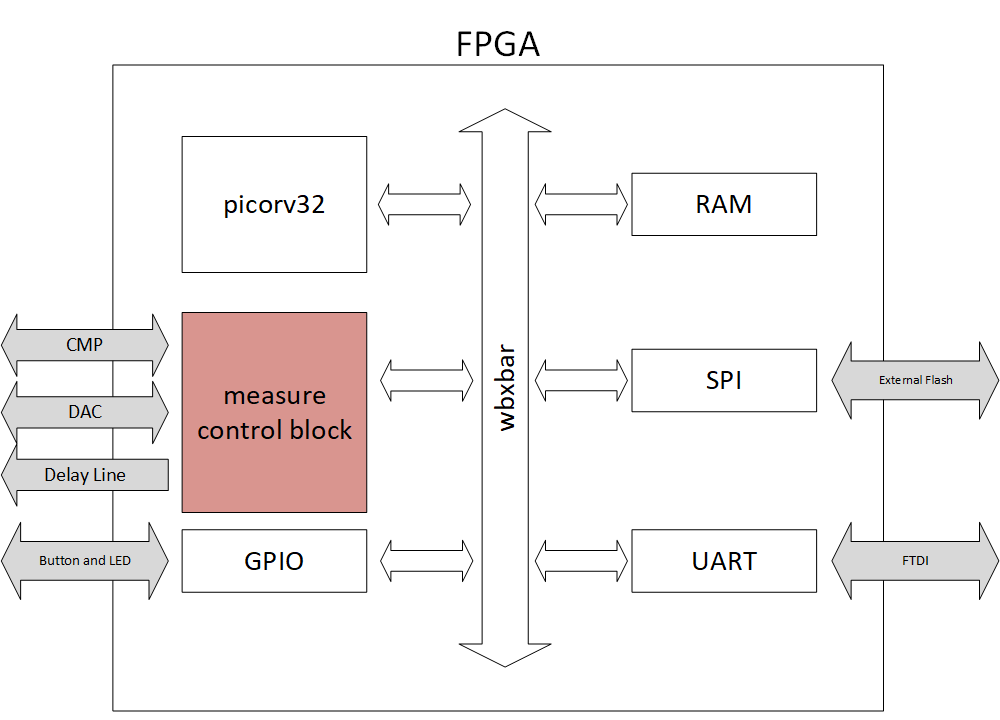
\includegraphics [scale=0.7] {my_folder/images//calsoc}
	\caption{Структурная схема СнК} 
	\label{fig:calsoc}  
\end{figure}

Все периферийные устройства разделяют между собой общее адресное пространство.

\begin{itemize}[label={}]
	\item 0x00000000 -- 0x00FFFFFF -- RAM 
	\item 0x01000000 -- 0x01FFFFFF -- ROM загрузичка
	\item 0x02000000 -- 0x02FFFFFF -- GPIO
	\item 0x03000000 -- 0x03FFFFFF -- UART1
	\item 0x04000000 -- 0x04FFFFFF -- память программы
	\item 0x05000000 -- 0x05FFFFFF -- измерительный модуль
\end{itemize}


\section{Измерительный модуль}

Измерительный модуль выдаёт все необходимые управляющие сигналы для проведения измерений и логически разделён на несколько компонентов (\firef{fig:mu-struct}):

\begin{itemize}
	\item \emph{stb\_gen} -- модуль, измеряющий частоту сигнала и генерирующий стробы
	\item \emph{ch\_measure\_ctl} -- модуль, непосредственно управляющий измерением одного канала
	\item \emph{spi\_master} -- модуль, реализующий взаимодействие с AD5662
	\item \emph{sc\_fifo} -- FIFO, накапливающее измеренные значения
\end{itemize}

\begin{figure}[ht!] 
	\center
	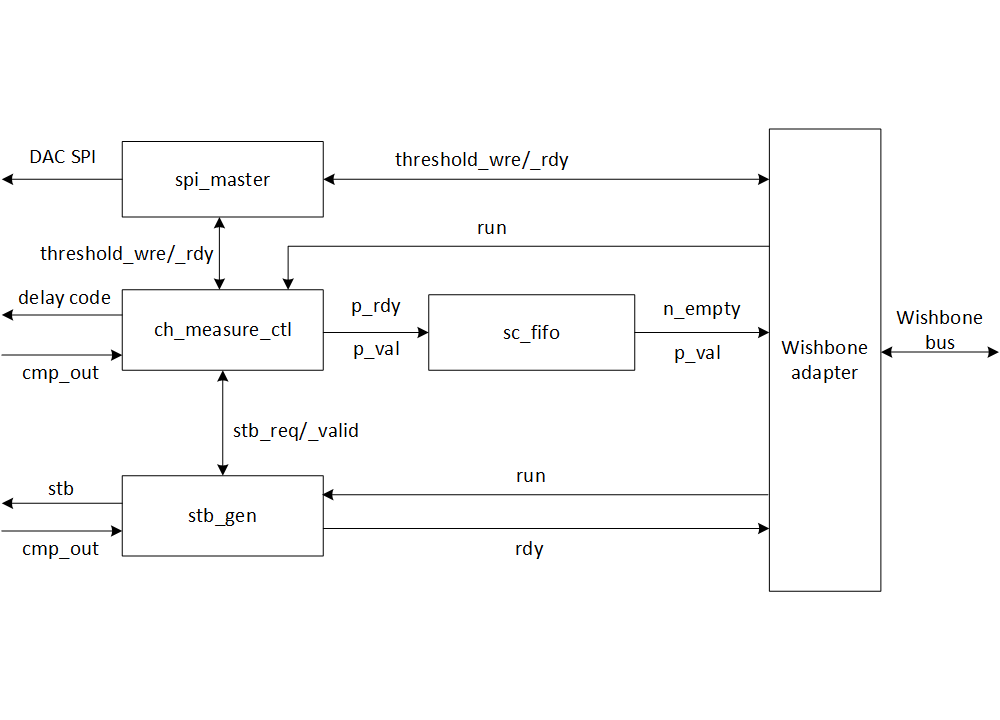
\includegraphics [scale=0.7] {my_folder/images//mu_struct}
	\caption{Структурная схема измерительного модуля (для одного канала)} 
	\label{fig:mu-struct}  
\end{figure}

Все описанные ранее модули подключены в модуле верхнего уровня \emph{measure\_unit}. В нём же
реализована вся логика управлением проведением измерений через шину Wishbone.

Далее будет отдельно рассмотрен каждый модуль.

\subsection{Модуль stb\_gen}

Для определения частоты измеряемого сигнала необходимо измерить время между двумя фронтами.
Для измерения используется 32-разрядный счётчик, один отсчёт которого равняется 8 нс (125 МГц).

Реализация <<в лоб>> не может работать стабильно на целевой ПЛИС из-за задержек на цепочке переносов в 
32-разрядном сумматоре. Для корректной работы на такой частоте необходимо конвейеризировать счётчик (\firef{fig:t-cnt}).

\begin{figure}[ht!] 
	\center
	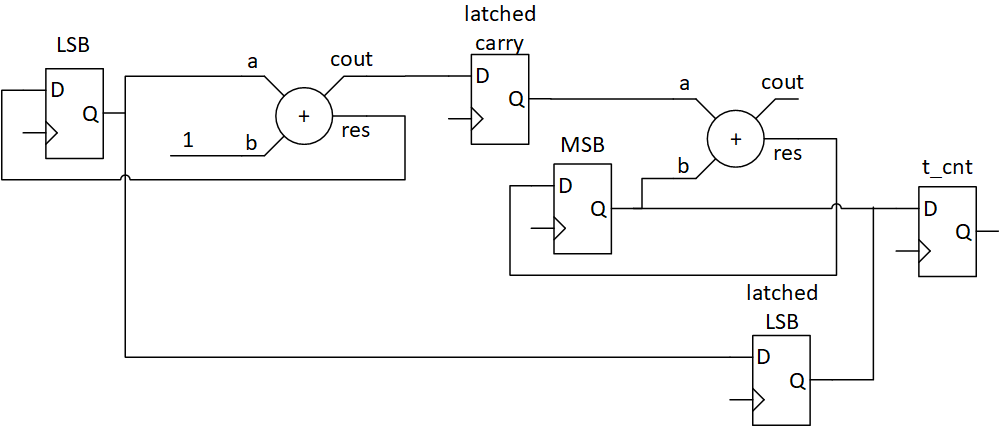
\includegraphics [scale=0.7] {my_folder/images//t_cnt}
	\caption{Конвейерный 32-х разрядный счётчик} 
	\label{fig:t-cnt}  
\end{figure}

К младшим байтам (регистр \emph{LSB}) каждый такт прибавляется 1, текущее значение младших байт защёлкивается в регистре \emph{latched LSB}.
При переполнении, перенос защёлкивается в регистре \emph{latched carry}. К старшим байтам (регистр \emph{MSB}) прибавляется сохранённый перенос из-за
младших байт. Выход счётчика -- комбинация значений регистров \emph{MSB} и \emph{latched LSB}.

\begin{flushright}
Листинг 3.1. Реализация на языке System Verilog
\end{flushright}
\lstset{
	numbersep = 5pt,
	stepnumber = 1
}
\begin{lstlisting}
// pipelined counter

	logic [T_CNT_WIDTH/2-1 : 0] high_bytes = 0;
	logic [T_CNT_WIDTH/2-1 : 0] latched_low_bytes = 0;
	logic [T_CNT_WIDTH/2-1 : 0] low_bytes = 0;
	logic [T_CNT_WIDTH/2-1 : 0] low_bytes_plus_1;
	logic carry;

	assign {carry, low_bytes_plus_1} = low_bytes + 1;

	//incrementing low bytes
	always_ff @(posedge clk_i, negedge arst_i) 
		if (~arst_i) low_bytes = 0;
		else low_bytes <= low_bytes_plus_1;

	//latching low bytes for 1 cycle
	always_ff @(posedge clk_i, negedge arst_i) 
		if (~arst_i) latched_low_bytes = 0;
		else latched_low_bytes <= low_bytes;

	logic latched_carry = 0;

	//latching carry
	always_ff @(posedge clk_i, negedge arst_i) 
		if (~arst_i) latched_carry = 0;
		else latched_carry <= carry;

	//adding latched carry to high bytes
	always_ff @(posedge clk_i, negedge arst_i)
		if (~arst_i) high_bytes = 0;
		else high_bytes <= high_bytes + latched_carry;

	//seting t_cnt
	always_ff @(posedge clk_i, negedge arst_i) 
		if (~arst_i) t_cnt = 0;
		else t_cnt <= {high_bytes, latched_low_bytes};
\end{lstlisting}

\begin{figure}[ht!] 
	\center
	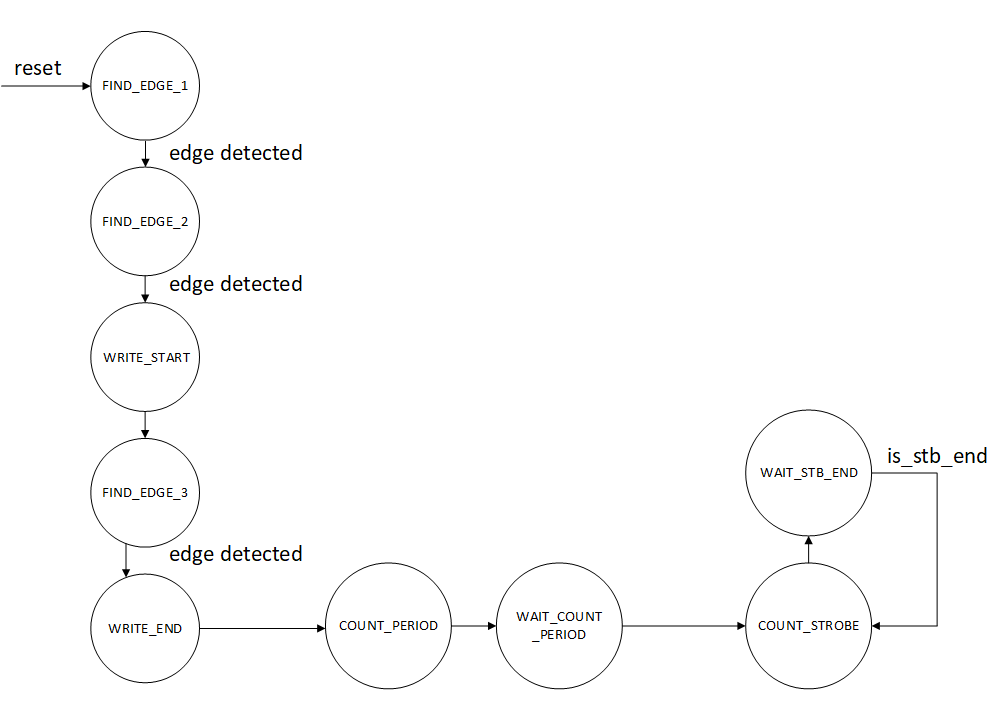
\includegraphics [scale=0.7] {my_folder/images//stb_gen_fsm}
	\caption{Конечный автомат модуля \emph{stb\_gen}} 
	\label{fig:stb-gen-fsm}  
\end{figure}

\FloatBarrier

Нас \firef{fig:stb-gen-fsm} представлен конечный автомат модуля \emph{stb\_gen}. Вся логика максимально упрощена, так как, если
на одной регистровой передаче будет много комбинаторной логики, при синтезе под целевую ПЛИС не получится выдержать требуемые $ t_{setup} $ и $ t_{hold} $.

\begin{itemize}[label={}]
	\item FIND\_EDGE\_1 -- состояние после сброса, ожидание первого фронта на входе \emph{sig\_i} 
	\item FIND\_EDGE\_2 -- ожидание второго фронта на входе \emph{sig\_i} 
	\item WRITE\_START -- запись текущего значения \emph{t\_cnt} в \emph{t\_start}
	\item FIND\_EDGE\_3 -- ожидание третьего фронта на входе \emph{sig\_i}
	\item WRITE\_END -- запись текущего значения \emph{t\_cnt} в \emph{t\_end}
	\item COUNT\_PERIOD -- вычисление периода сигнала ($ \emph{t\_end} - \emph{t\_start}) $
	\item WAIT\_COUNT\_PERIOD -- задержка на 1 такт
	\item COUNT\_STROBE -- начало расчёта времени начала и конца отрицательного импульса на выходе стробы
	\item WAIT\_STB\_END -- ожидание конца стробы и переход к расчёту новой\\
\end{itemize}

Таким образом, модуль определяет частоту входного сигнала и начинает бесконечно выдавать стробы.

Помимо 32-х разрядного счётчика, конвейеризация была необходима для всех операций с 32-х битными числами. В модуле \emph{two\_cycle\_32\_adder}
реализован двухтактный сумматор, однако использованный подход идентичен тому, что используется в счётчике.

Отдельного упоминания стоит оптимизация операции проверки на равенство двух чисел. Для этого необходимо сравнить попарно все биты
чисел, что выполняется параллельно и не должно увеличивать максимальный путь, однако при синтезе получалась цепочка с последовательным
сравнением всех разрядов (\firef{fig:eq}).\\

\begin{figure}[ht!] 
	\center
	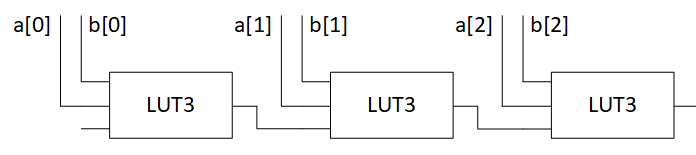
\includegraphics [scale=0.7] {my_folder/images//eq}
	\caption{Реализация сравнения при синтезе} 
	\label{fig:eq}  
\end{figure}

\FloatBarrier

Для исправления этого пришлось явно заменить операцию сравнения на исключающее ИЛИ и свёртку по ИЛИ-НЕ.

\begin{flushright}
Листинг 3.2. Реализация сравнения
\end{flushright}
\lstset{
	numbersep = 5pt,
	stepnumber = 1
}
\begin{lstlisting}
always_ff @(posedge clk_i) is_zero_hold_start_lo <=  ~|(t_cnt[15:0] ^ latched_zero_hold_res[15:0]);  //t_cnt == latched_zero_hold_res;
	always_ff @(posedge clk_i) is_zero_hold_start_hi <=  ~|(t_cnt[31:16] ^ latched_zero_hold_res[31:16]);  //t_cnt == latched_zero_hold_res;
	always_ff @(posedge clk_i) is_zero_hold_start <= is_zero_hold_start_lo & is_zero_hold_start_hi; 
\end{lstlisting}

При работе модуль не выдаёт стробы, а держит компаратор в защёлкнутом состоянии. Для запроса стробы используется пара сигналов
\emph{stb\_req\_i} и \emph{stb\_valid\_o}. При выдаче стробы, с компаратора снимается защёлка на короткое время, после чего устанавливается обратно.

Для тестирования модуля были написаны тестбенчи \emph{tb\_stb\_gen.sv} и \emph{tb2\_stb\_gen.sv}. На \firef{fig:tb-stb-gen} и \firef{fig:tb-stb-gen-out}
представлены результаты моделирования.

\begin{figure}[ht!] 
	\center
	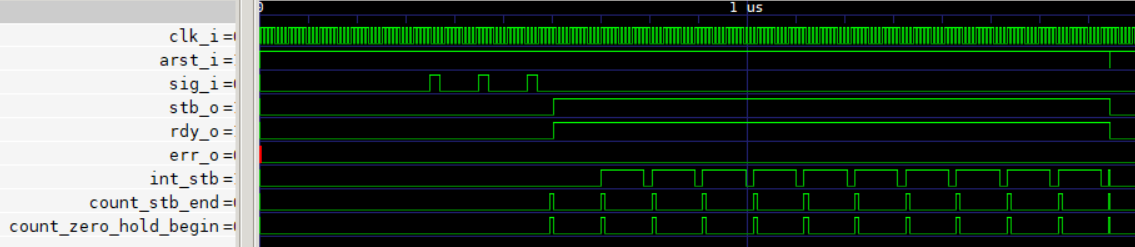
\includegraphics  [scale=0.7] {my_folder/images//tb_stb_gen}
	\caption{Пример определения частоты входного сигнала} 
	\label{fig:tb-stb-gen}  
\end{figure}

\begin{figure}[ht!] 
	\center
	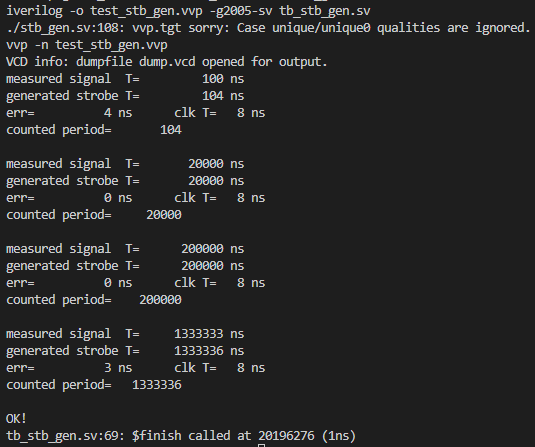
\includegraphics  [scale=0.8] {my_folder/images//tb_stb_gen_out}
	\caption{Вывод в консоль при симуляции} 
	\label{fig:tb-stb-gen-out}  
\end{figure}
\FloatBarrier

Видно, что сигналы с периодом, кратным 8 нс измеряются корректно, при измерении других -- ошибка меньше 8 нс.

\begin{figure}[ht!] 
	\center
	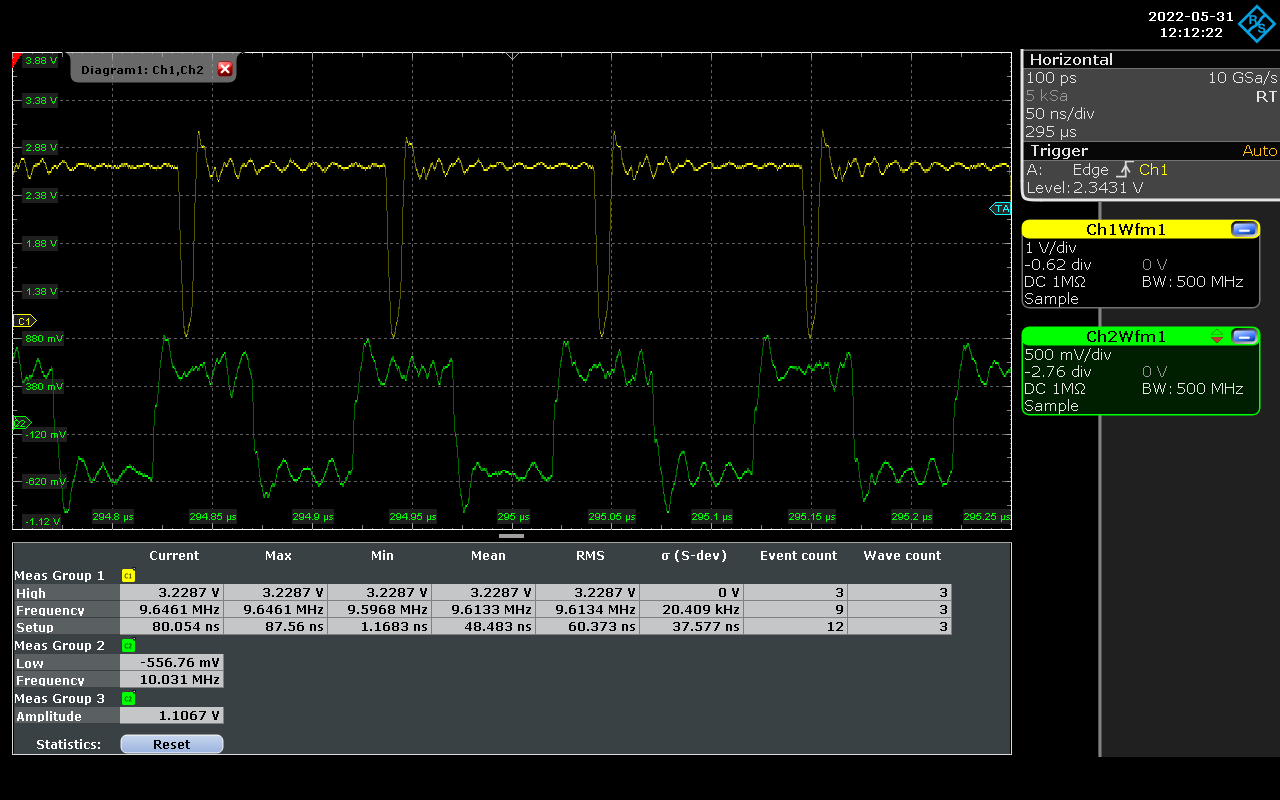
\includegraphics  [scale=0.3] {my_folder/images//stb_10mhz}
	\caption{Генерация строб для 10 Мгц} 
	\label{fig:stb-10mhz}  
\end{figure}

\begin{figure}[ht!] 
	\center
	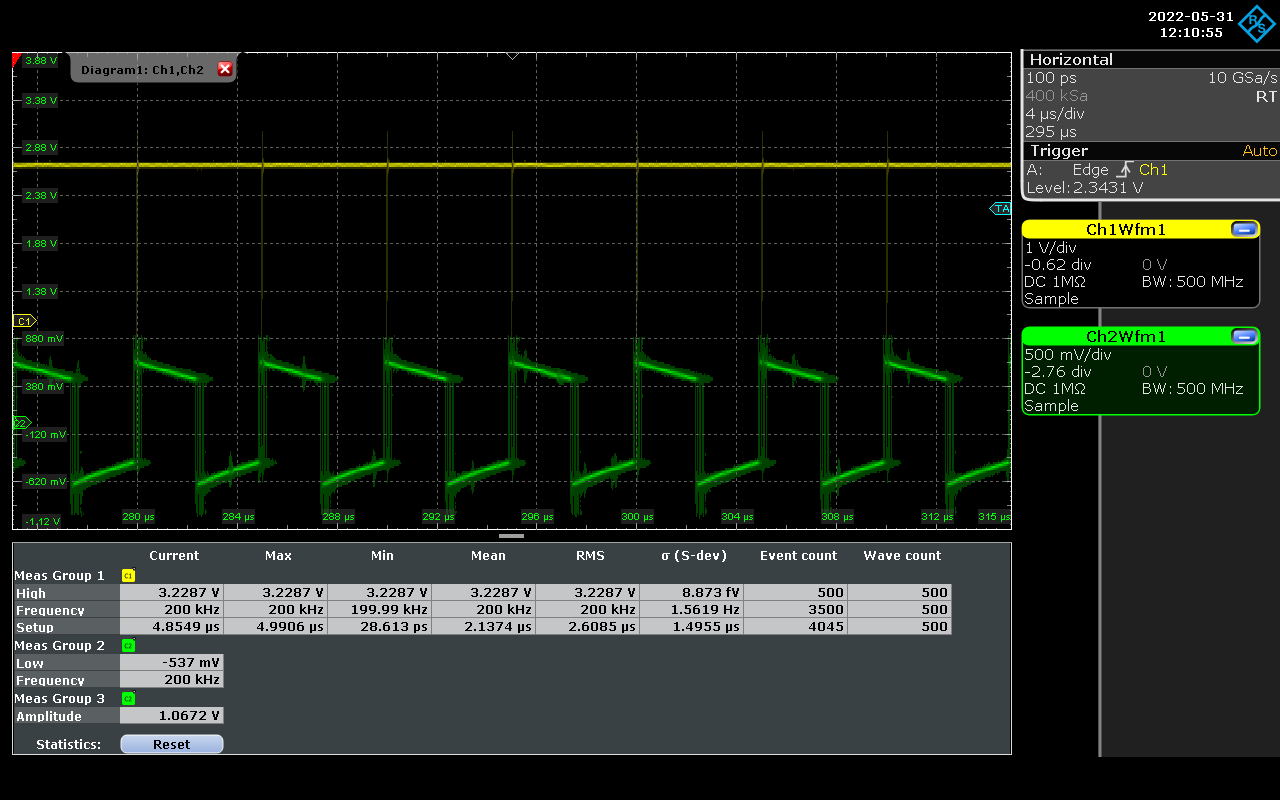
\includegraphics  [scale=0.3] {my_folder/images//stb_200khz}
	\caption{Генерация строб для 200 кГц} 
	\label{fig:stb-200khz}  
\end{figure}

\FloatBarrier

На \firef{fig:stb-10mhz} и \firef{fig:stb-200khz} приведены осциллограммы генерации строб для 10 МГц и 200 кГц.
Видно, что точно определить не кратную частоту невозможно -- при генерации получается стробы с частотой 9.6 Мгц, а не 10 Мгц.

\subsection{Модуль \emph{ch\_measure\_ctl}}

Данный модуль управляет измерением одного из каналов -- выставляет необходимое пороговое напряжение и задержку, а
затем выставляет запрос на стробу. После прохода стробы, в зависимости от текущего и предыдущего выхода компаратора, принимается решение
о следующем значении задержки и порогового напряжения.

Для ускорения снятия осциллограммы применяется предсказание направления изменения сигнала. Для этого, после нахождения очередной точки,
изменяется только задержка, после чего на основании выхода компаратора принимается решение -- измеряемый сигнал нарастает или уменьшается.

\begin{figure}[ht!] 
	\center
	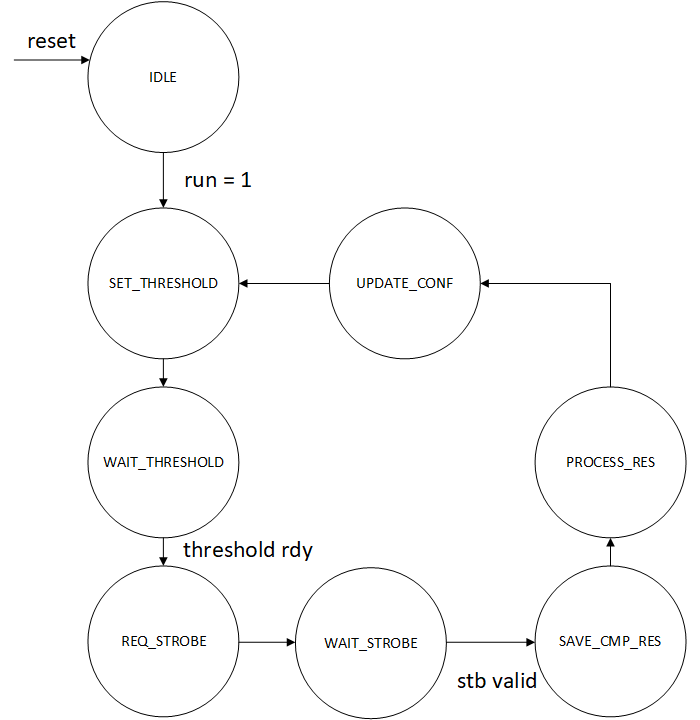
\includegraphics  [scale=0.7] {my_folder/images//ch_ctl}
	\caption{Конечный автомат модуля \emph{ch\_measure\_ctl}} 
	\label{fig:ch-ctl-fsm}  
\end{figure}

\FloatBarrier

На \firef{fig:ch-ctl-fsm} представлен конечный автомат описываемого модуля.

\noindent
\begin{itemize}[label={}]
	\item IDLE -- состояние покоя 
	\item SET\_THRESHOLD -- отправление запроса на установку порогового напряжения ($ \emph{threshold\_wre\_o} = 1 $)
	\item WAIT\_THRESHOLD -- ожидание установки порогового напряжения ($ \emph{threshold\_rdy\_i} == 1 $)
	\item REQ\_STROBE -- установка запроса на стробу ($ \emph{stb\_req\_o} = 1 $)
	\item WAIT\_STROBE -- ожидание прохода стробы ($ \emph{stb\_valid\_i} == 1 $)
	\item SAVE\_CMP\_RES -- обновление текущего и предыдущего выхода компаратора
	\item PROCESS\_RES -- принятие решения о статусе поиска точки (определение направления поиска или поиск точки)
					и о выборе направления поиска
	\item UPDATE\_CONF -- обновление регистров с текущей задержкой и пороговым напряжением на основании принятого ранее решения\\
\end{itemize}

В состоянии PROCESS\_RES, в зависимости от выхода компаратора переключаются два других конечных автомата, отвечающих за статус поиска точки и направления поиска.

На \firef{fig:p-find} приведён пример снятия осциллограммы сигнала.

\begin{figure}[ht!] 
	\center
	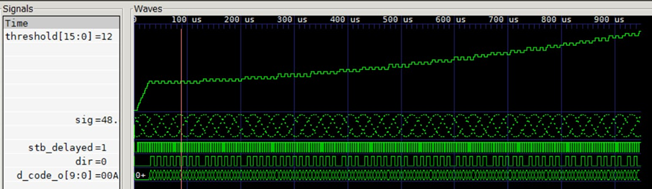
\includegraphics  {my_folder/images//p_find}
	\caption{Пример снятия осциллограммы с угадыванием направления изменения сигнала} 
	\label{fig:p-find}  
\end{figure}



\newpage